\documentclass[../main.tex]{subfiles}
\graphicspath{{\subfix{../figures/}}}
%
\title{知识结构化}
%
\begin{document}
\maketitle
%
\section{引子}
在个人知识管理流程中,知识结构化是知识提炼环节的一个要点。
简单的收藏,并不代表拥有了知识;快速阅读一遍,内化的知识只怕也有限。
只有掌握了知识的内部结构,进而与已有的知识网络发生联系,才是有效的学习。
%
\subsection{本文讨论的范围}
广义上,知识包括数据、信息、知识。

根据研究目的和对象的不同,对数据结构的要求也不一样,
这通常是专业分析和计算机处理才要考虑的问题。

美国信息管理专家霍顿(F.W.Horton)认为:
``信息是为了满足用户决策的需要而经过加工处理的数据。''

也就是说,信息依附于决策模型之后,作为方法论与现实世界问题的连接。
因此,只要确定好方法论与规律的结构,信息的存放位置也就能够确定。

这些规律与方法论就是我们所称的狭义的知识。
由于它们会被重复使用,因此结构化若能提升学习、运用知识的效率,
就会给我们带来巨大收益。
%
\begin{itemize}
  \item 信息是这里有一瓶水,现在是七度,是\textbf{外部的一个客观事实},
    这是一个\textbf{信息}。
  \item 水在零度的时候会结冰,这是一个\textbf{知识},
    是\textbf{对外部客观规律的归纳和总结}。
  \item 在未来的时间中我在什么时候把什么味道的水变成什么味道的冰棒,
    卖给谁叫做\textbf{智慧和能力},它是指\textbf{对知识的处理和运用}。
\end{itemize}
%
本文重点探讨这些能揭示规律、指导行为的知识的结构化。
%
\section{为什么要结构化}
我们依赖分类和结构认知世界,
人类有两种认知形式,一种是\textbf{自下而上},一种是\textbf{自上而下}。
\\

\begin{cuenotes}
  \cue{自下而上}
  \note{
    自下而上的知觉是基于具体的、细节的感知,
    采用分类的认知方法---将事物拆解为一些基本的概念。
  }
  \note{
    我们来做个实验,看下图,然后思考你是如何辨认图中生物的:
    \begin{figure}[H]
      \begin{center}
        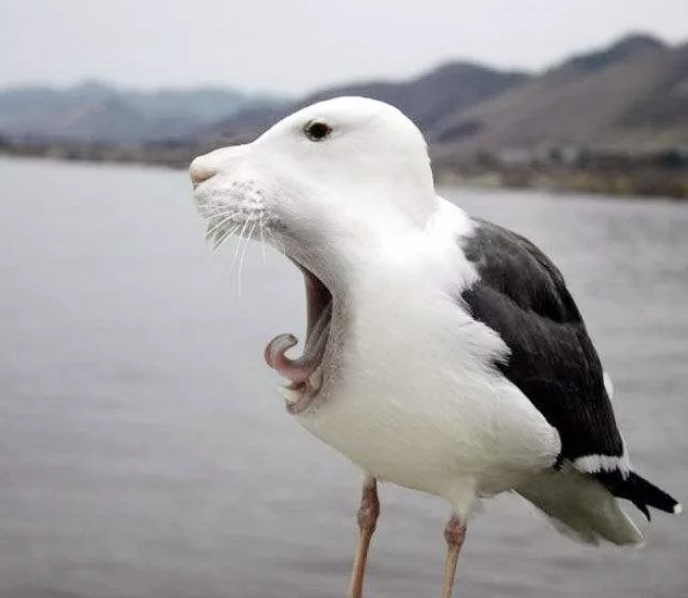
\includegraphics[width=0.50\textwidth]{animal.png}
      \end{center}
    \end{figure}
    由于一眼看上去不像是熟知的物种,于是你仔细辨认:
    兽类的嘴,覆盖身上的羽毛,鸟类的尾巴和双脚。
  }
  \note{
    要认识没见过的事物,我们不得不把它拆解为一些简单的基本概念,
    比如兽嘴、羽毛、鸟尾。我们称这些基本概念为``几何子''。
    吉利汽车李书福曾说过一句很有名的话:
    ``轿车不就是四个轮子,几个沙发,加上一个铁壳吗?''
    这番言论很形象地反映了这类知觉的特点。
  }
  \cue{自上而下}
  \note{
    当我们观察熟悉的事物时,却不需要分析成分,
    而依赖如同预制模块般的先验知识。
    比如我们可能不知道轿车,但是我们太熟悉轮子了,当我们看待轮子时,
    就不会将它进一步分解为轮胎、轮毂、辐条、中心轴这些更基本的构件,
    而是从整体上去把握。
    这种整体性而不是分析性的认知模式大大提升了我们的认知效率。
    这就是自上而下,一种``模块化''的知觉形式。
  }
\end{cuenotes}
%
\subsection{语言有内在结构}
除了通过直接经验学习,人类还通过语言文字继承知识。

语言自有其内在结构。一篇长文,
我们知道如何区分起、承、转、合,知道哪些是论点,哪些是证据。
一个句子,我们可以分出来主、谓、宾、定、状、补。
语义和排列方式共同决定了各个成分之间的关系,
使得我们在线性文本中读出篇章结构和句子结构。
%
\begin{figure}[H]
  \begin{center}
    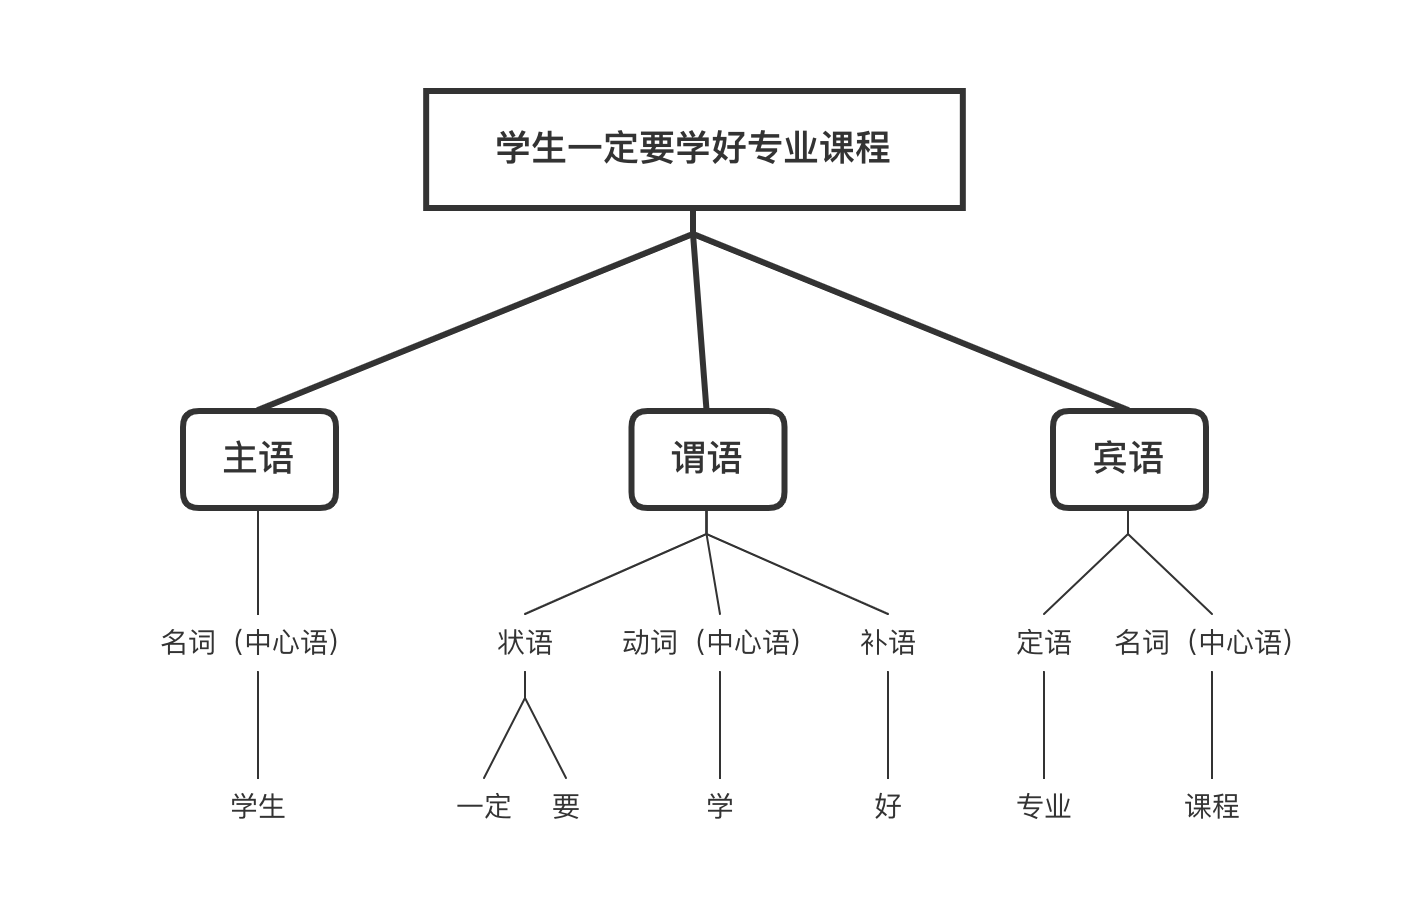
\includegraphics[width=0.55\textwidth]{语言的内在结构.png}
  \end{center}
\end{figure}
%
认知科学家把人类的记忆建模成由许多节点结合而成的网络。
而斯蒂芬·平克认为,人类输出语言是运用句法树将大脑中的思维网转换为词语串的过程。
输入语言则相反。
%
\begin{figure}[H]
  \begin{center}
    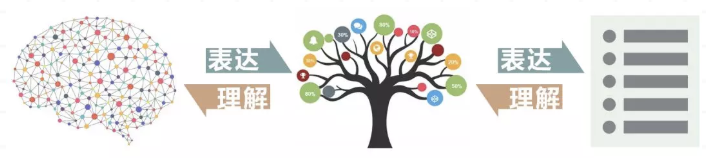
\includegraphics[width=0.55\textwidth]{输入与输出语言.png}
  \end{center}
\end{figure}
%
那么,如果能够舍去词语串,不就可以节省一个环节吗?
当用口语表达时,由于只能在时间线上铺开,采用线性的词语串不可避免。
但若是用于书面展示,何不考虑直接以``句法树''、``篇章结构树''的形态呈现?

我们可以用一个例子来展示清晰的语言结构如何帮助我们理解和思考。

逻辑评价的重要技术之一,就是将论证改写成``良构论证''的标准形式,
让重要的逻辑特征得到明确陈述:前提是什么,子结论是什么,
最终结论又是什么。
更进一步,还要求消除冗词、使用一致的语言。
因为语言的模糊和混乱会干扰思维,增加评价的难度。
良构论证,本质就是一种标准化的语言结构。

综上所述,认知未见过的事物时,我们需要借助分类;
认知已知的事物时,模块化可以帮助我们降低认知负载。
书面文字如果保留在理解过程的中间状态——``语法树'',
将有助于增加理解的流畅性。

如果一种书面结构,能让知识的呈现符合大脑的认知规律,
将会提升阅读和学习的效率。
%
\section{常用的知识结构}
常用的知识结构有两种:\textbf{分类结构}和\textbf{关系结构}。
%
\subsection{分类结构}
\begin{cuenotes}
  \cue{二维分类}
  \note{
    二维表(或称二维矩阵)在横向和纵向各使用一个属性进行分类,
    形成交叉,每一个格子对应两项属性。例如著名的时间管理矩阵。
    \begin{figure}[H]
      \begin{center}
        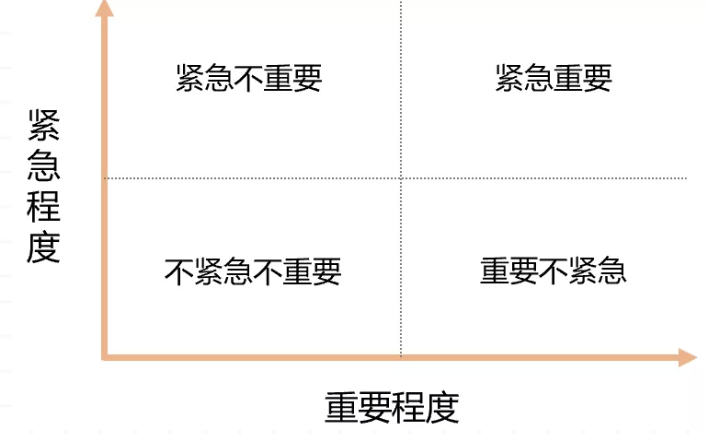
\includegraphics[width=0.80\textwidth]{time_matrix.png}
      \end{center}
    \end{figure}
  }
  \cue{一维分类(每次只在一个属性上进行分类,多个属性就需要多层分类。)}
  \note{
    \textbf{大纲}: \\
    \begin{figure}[H]
      \begin{center}
        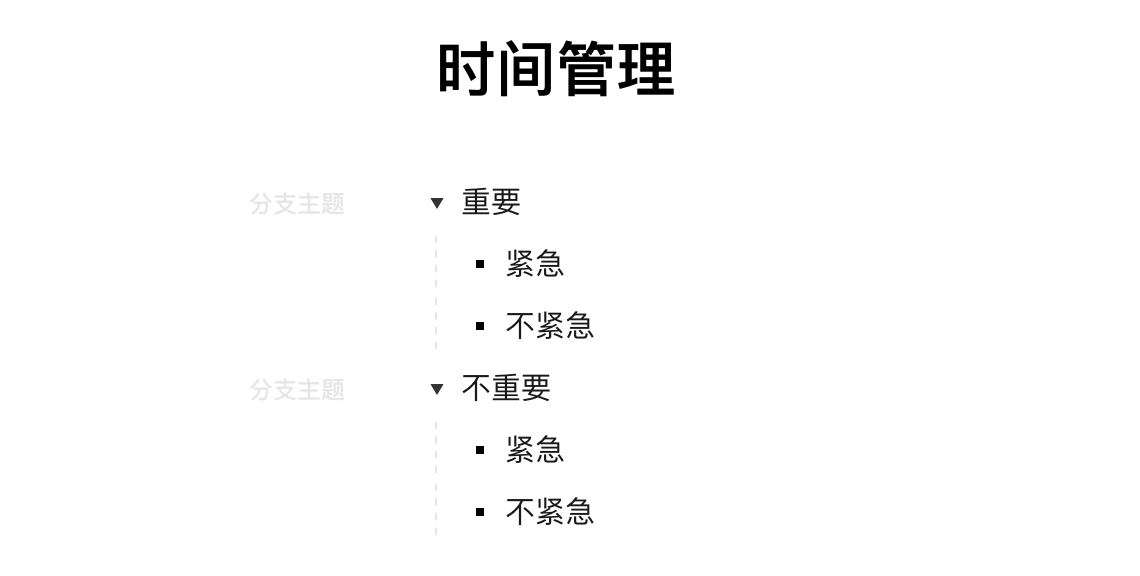
\includegraphics[width=0.80\textwidth]{time_outline.png}
      \end{center}
    \end{figure}
    大纲的优点是不占横向空间,适合在手机上使用,
    但是在结构呈现上远不如思维导图清晰,尤其是列表特别长的时候。
  }
  \note{
    \textbf{思维导图}: \\
    \begin{figure}[H]
      \begin{center}
        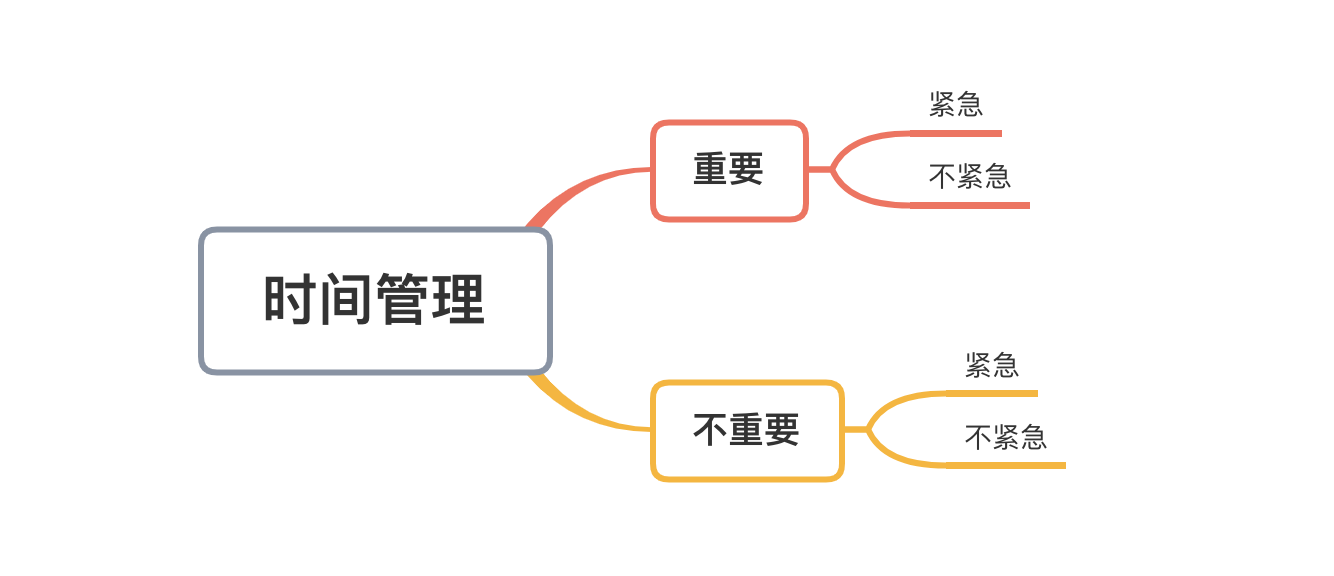
\includegraphics[width=0.80\textwidth]{time_mindmap.png}
      \end{center}
    \end{figure}
    思维导图结构一目了然,缺点是不适合小屏阅读。
    另外过于庞杂会让思维导图失去良好的阅读体验,
    因此必须有一定的规则和策略进行约束。
  }
  \note{
    \textbf{韦恩图}(直观表现两个概念的关系): \\
    \begin{figure}[H]
      \begin{center}
        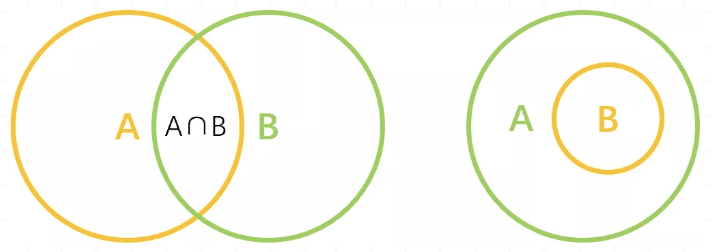
\includegraphics[width=0.80\textwidth]{venn.png}
      \end{center}
    \end{figure}
  }
  \note{
    可见在表现交叉属性的时候,一维分类效果不如二维分类。
    一维分类只能先分一个属性,再分另一属性,
    而二维分类阅读者可以任意选择一维切入。
  }
  \note{
    另外也显示出思维导图与大纲的区别:结构上完全一样(都是树状图),
    只是表现形式不一样。
    大纲一行一行向下伸展,通过缩进体现层级。
    典型的思维导图横向拓展层级,纵向铺开同级要点。
  }
\end{cuenotes}
%
\subsection{关系结构}
\begin{cuenotes}
  \cue{相关关系}
  \note{
    概念图:
    \begin{figure}[H]
      \begin{center}
        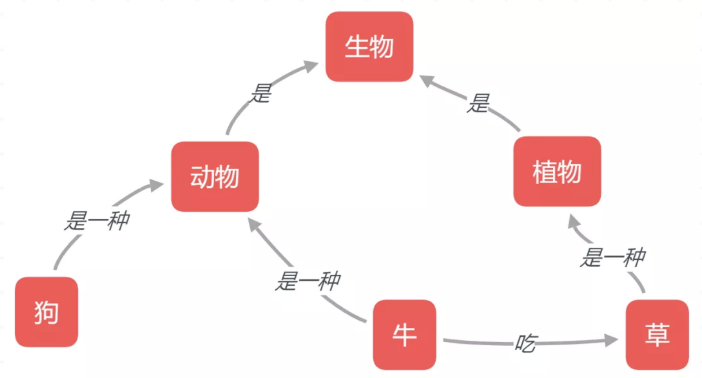
\includegraphics[width=0.80\textwidth]{概念图.png}
      \end{center}
    \end{figure}
    概念图的编制通常是先列出多个相关概念,
    然后努力发掘概念之间的关系,进行连线,
    并在线上标记关系内容。
  }
  \note{
    知识图谱:
    \begin{figure}[H]
      \begin{center}
        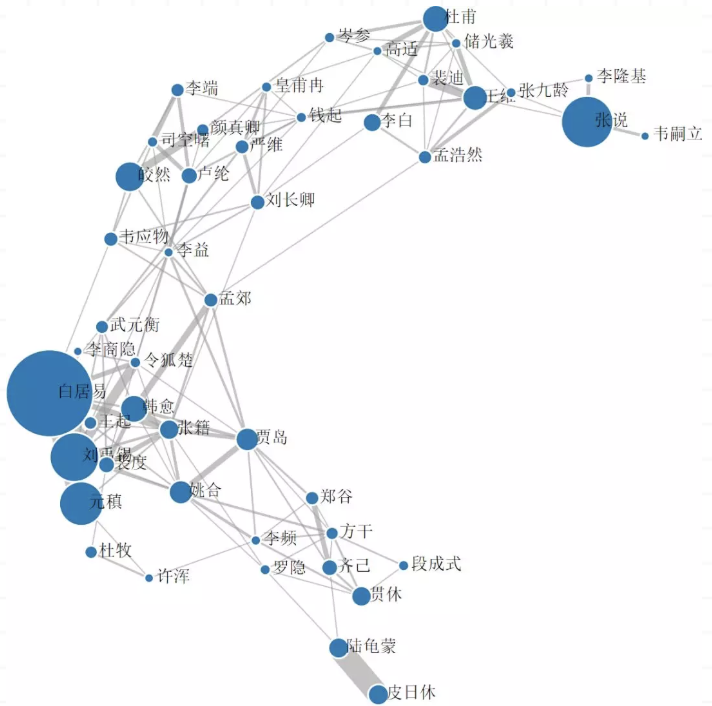
\includegraphics[width=0.80\textwidth]{知识图谱.png}
      \end{center}
    \end{figure}
    知识图谱由人工录入或计算机自动从文本提取节点及关系信息,
    节点相互连接,从而形成知识网络结构。
    知识图谱通过图分析工具实现可视化,
    可以看成一种通过节点关系自动生成的概念图,
    优点在于可以展示节点及关系的权重。
  }
  \cue{因果关系}
  \note{
    系统图:
    \begin{figure}[H]
      \begin{center}
        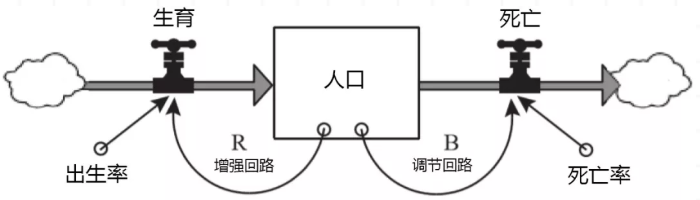
\includegraphics[width=0.80\textwidth]{系统图.png}
      \end{center}
    \end{figure}
    系统图(存量流量图)通常由存量、流量,以及调节回路、增强回路构成,
    用以描述一个自然系统或社会系统的要素、关系及动态过程。
  }
  \cue{先后顺序}
  \note{
    流程图:
    \begin{figure}[H]
      \begin{center}
        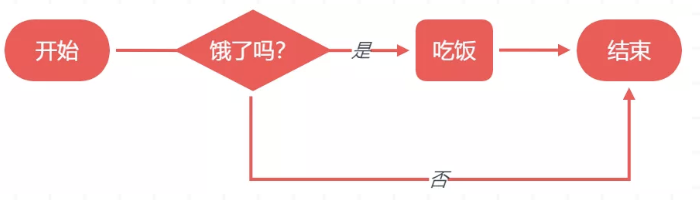
\includegraphics[width=0.80\textwidth]{流程图.png}
      \end{center}
    \end{figure}
    流程图直观地描述一个流程的具体步骤,揭示如何从``开始''到``结束''。
  }
\end{cuenotes}
%
\subsection{哪种知识结构更好?}
事实是,每一种知识结构各有其作用。

模块化是有效的认知手段。

系统图、流程图、韦恩图、二维表是各自类型知识模块的最佳呈现方式,
但是使用范围都比较窄。二维表是一种清晰稳定的结构,
且有成熟的统计分析工具,但相对来说比较僵化,缺少自由度,
适合有固定格式的数据和信息的长期记录。

分类是最普遍的思维。

树状图是比韦恩图、二维表使用更灵活,适用范围更广的层级分类结构。
树状图围绕中心概念或命题层层发散,有清晰的焦点,
构成一个完整的知识模块,同时可以清晰辨别支持中心主题的次级模块、
次次级模块……因此,树状图尤其是思维导图既符合认知的分类和模块化的特点,
同时又能在空间上还原语言的树状结构,
看起来是最具有普遍适用性的一种知识结构。
实际使用时可以灵活组合,将思维导图作为一个基础的知识架构,
在合适的节点以图片或附件形式插入上述其他结构。

那么概念图呢?在概念图中,由于每一个概念只出现一次,常常导致连线交叉,
视觉混乱,并不容易看清分组;可以发现聚集的概念群落,
而不易于展示清晰的知识模块。

概念图更适用于表现概念关系,并判断概念在关系网中的作用和地位。
从一个更高的视角俯视概念群,可以获得更全面的认识,
从而挖掘更高维度的知识。但是深入理解概念最好通过中心发散的思维导图。

好比人类观察世界,当寻求更开阔的视野,将眼角余光都利用起来,
实际上只能获得一种朦胧的观感。唯有聚焦,才能真正看清楚。

思维导图正是这种提供理解焦点的知识呈现形式。
只有在更为抽象的层面思考时,
才考虑用概念图将思维导图所表述的中心概念串联起来。
%
\subsection{结构化的细节与补充}
下面的补充主要针对思维导图,但是其他类型的知识结构多数可以参考,
原则都是相通的。
\\

\begin{cuenotes}
  \cue{用语简洁}
  \note{
    用尽可能少的字讲清楚知识。
    这是一个压缩信息的过程,越简洁越凸显要点,也越容易重复使用。
  }
  \cue{把握焦点,划定边界}
  \note{
    有时候会不自觉把一张图做得很大,不断扩展,内容丰富。
    但是过于庞杂容易失去焦点,在屏幕上四处腾挪着阅读也不方便。
    因此,除了用语简洁,不要妄图用一张图涵盖所有知识,
    要针对特定的焦点主题,划定边界。
    重要的支持模块另起一张图,再把它们链接起来。
  }
  \cue{设置路标,快速定位}
  \note{
    路标是提纲挈领的用语,可以是提炼出来的共同属性或关键词。
    做好分类、归纳,让知识更具层次。
  }
  \cue{前后一致性}
  \note{
    相同类型的主题采用相同的诠释框架。
    尽量使用一致的顺序,一致的用语,一致的图标。
  }
  \cue{全文检索}
  \note{
    对于任何知识管理系统来说,全文检索都是十分重要的功能。
  }
\end{cuenotes}

\textbf{知识结构化的意义}:
%
\begin{itemize}
  \item 借助各类结构提炼出简洁清晰可复用的知识模型;
  \item 借助思维导图结构实现快速回顾知识;
  \item 节省下认知资源用于更高层次的思考;
  \item 通过树状结构层层拆解知识,小颗粒度的知识模块更容易进行重组,
    提高了知识创新的效率。
\end{itemize}
%
⇲\textbf{参考资料}:
%
\begin{itemize}
  \item 《风格感觉》,[美] 史蒂芬·平克
  \item 《认知心理学》,E. Bruce Goldstein
  \item 《系统之美》,Wright, Diana; Meadows, Donella H.
  \item 《学习、创造与使用知识:概念图促进企业和学校的学习变革》,
    [美] Joseph D.Novak
\end{itemize}
%
\end{document}
